% \title{Assignment 03 of Automata Theory}

%%%%%%%%%%%%%%%%%%%%%%%%%%%%%%%%%%%%%%%%%
% Short Sectioned Assignment
% LaTeX Template
% Version 1.0 (5/5/12)
%
% This template has been downloaded from:
% http://www.LaTeXTemplates.com
%
% Original author:
% Frits Wenneker (http://www.howtotex.com)
%
% License:
% CC BY-NC-SA 3.0 (http://creativecommons.org/licenses/by-nc-sa/3.0/)
%
%%%%%%%%%%%%%%%%%%%%%%%%%%%%%%%%%%%%%%%%%

% -----------------------------------------------------------------------------
% PACKAGES AND OTHER DOCUMENT CONFIGURATIONS
% -----------------------------------------------------------------------------

\documentclass[paper=a4, fontsize=11pt]{scrartcl} % A4 paper and 11pt font size

\usepackage[T1]{fontenc} % Use 8-bit encoding that has 256 glyphs
\usepackage{fourier} % Use the Adobe Utopia font for the document - comment this line to return to the LaTeX default
\usepackage[english]{babel} % English language/hyphenation
\usepackage{amsmath,amsfonts,amsthm,amssymb} % Math packages
\usepackage{graphicx}

\usepackage{sectsty} % Allows customizing section commands
\allsectionsfont{\centering \normalfont\scshape} % Make all sections centered, the default font and small caps

% --------------------
% Quote Style
% --------------------

\usepackage{tikz}
\usetikzlibrary{backgrounds}
\makeatletter

\tikzset{%
  fancy quotes/.style={
    text width=\fq@width pt,
    align=justify,
    inner sep=.2em,
    anchor=north west,
    minimum width=\textwidth,
  },
  fancy quotes width/.initial={.8\textwidth},
  fancy quotes marks/.style={
    scale=2,
    text=white,
    inner sep=0pt,
  },
  fancy quotes opening/.style={
    fancy quotes marks,
  },
  fancy quotes closing/.style={
    fancy quotes marks,
  },
  fancy quotes background/.style={
    show background rectangle,
    inner frame xsep=0pt,
    background rectangle/.style={
      fill=gray!25,
      rounded corners,
    },
  }
}

\newenvironment{fancyquotes}[1][]{%
  \noindent
  \tikzpicture[fancy quotes background]
  \node[fancy quotes opening,anchor=north west] (fq@ul) at (0,0) {$``$};
  \tikz@scan@one@point\pgfutil@firstofone(fq@ul.east)
  \pgfmathsetmacro{\fq@width}{\textwidth - 2*\pgf@x}
  \node[fancy quotes,#1] (fq@txt) at (fq@ul.north west) \bgroup}
{\egroup;
  \node[overlay,fancy quotes closing,anchor=east] at (fq@txt.south east) {''};
  \endtikzpicture}

\makeatother

% --------------------
% Header and Footer
% --------------------

\usepackage{fancyhdr} % Custom headers and footers
\pagestyle{fancyplain} % Makes all pages in the document conform to the custom headers and footers
\fancyhead[L]{\normalfont \normalsize \textsc{Automata Theory}} % Class
\fancyhead[R]{\normalfont \normalsize \textsc{Wanzhang Sheng}} % Author
\fancyfoot[L]{} % Empty left footer
\fancyfoot[C]{} % Empty center footer
\fancyfoot[R]{\thepage} % Page numbering for right footer
\renewcommand{\headrulewidth}{0pt} % Remove header underlines
\renewcommand{\footrulewidth}{0pt} % Remove footer underlines
\setlength{\headheight}{13.6pt} % Customize the height of the header

\numberwithin{equation}{section} % Number equations within sections (i.e. 1.1, 1.2, 2.1, 2.2 instead of 1, 2, 3, 4)
\numberwithin{figure}{section} % Number figures within sections (i.e. 1.1, 1.2, 2.1, 2.2 instead of 1, 2, 3, 4)
\numberwithin{table}{section} % Number tables within sections (i.e. 1.1, 1.2, 2.1, 2.2 instead of 1, 2, 3, 4)

\setlength\parindent{0pt} % Removes all indentation from paragraphs - comment this line for an assignment with lots of text

% -----------------------------------------------------------------------------
% TITLE SECTION
% -----------------------------------------------------------------------------

\newcommand{\horrule}[1]{\rule{\linewidth}{#1}} % Create horizontal rule command with 1 argument of height

\title{
  \horrule{0.5pt} \\[0.4cm] % Thin top horizontal rule
  \huge Assignment 03 \\ % The assignment title
  \horrule{2pt} \\[1.0cm] % Thick bottom horizontal rule
}

\author{Wanzhang Sheng} % Your name

\date{\normalsize\today} % Today's date or a custom date

\begin{document}

\maketitle % Print the title

% -----------------------------------------------------------------------------
% PROBLEM 1
% -----------------------------------------------------------------------------
\section{}

\begin{fancyquotes}
  Give a DFA for each of the following languages:
\end{fancyquotes}

\begin{enumerate}
\item
  \begin{fancyquotes}
    (4 points) All strings over $\{a, b, c\}$ that contain an even number
    of $a$'s
  \end{fancyquotes}

  \begin{figure}[hp]
    \centering
    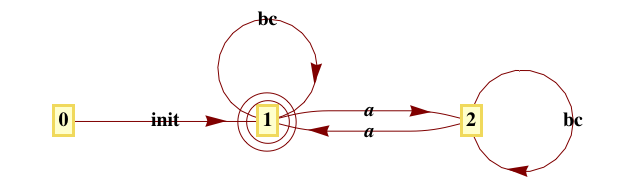
\includegraphics[width=1.0\textwidth]{1-1}
    \caption{All strings over $\{a, b, c\}$ that contain an even
      number of $a$'s}
  \end{figure}

\item
  \begin{fancyquotes}
    (4 points)All strings over $\{a, b, c\}$ that contain an even
    number of $a$'s and an even number of $b$'s
  \end{fancyquotes}

  \begin{figure}[hp]
    \centering
    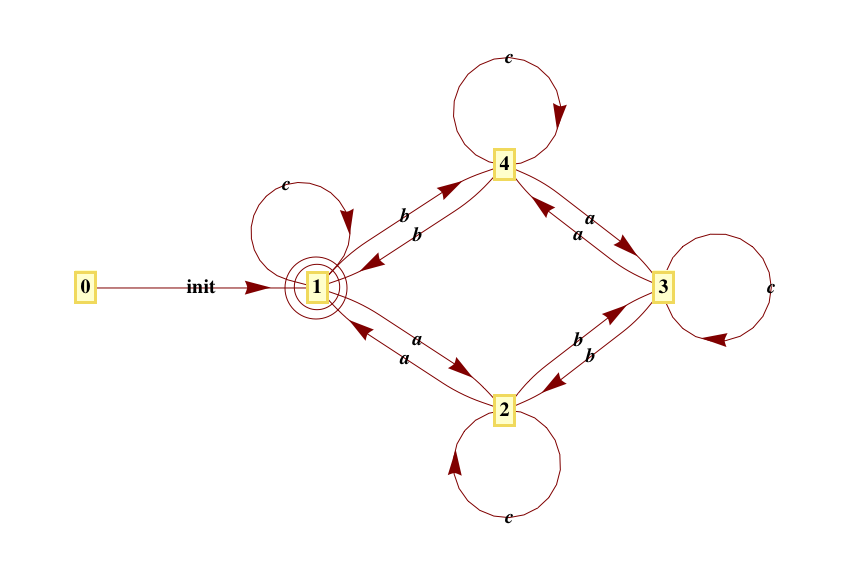
\includegraphics[width=1.0\textwidth]{1-2}
    \caption{All strings over $\{a, b, c\}$ that contain an even number of $a$'s and an even number of $b$'s}
  \end{figure}

\item
  \begin{fancyquotes}
    (4 points) All strings over $\{a,b\}$ that contain either $aab$ or $bba$
    (or both)
  \end{fancyquotes}
  \begin{figure}[hp]
    \centering
    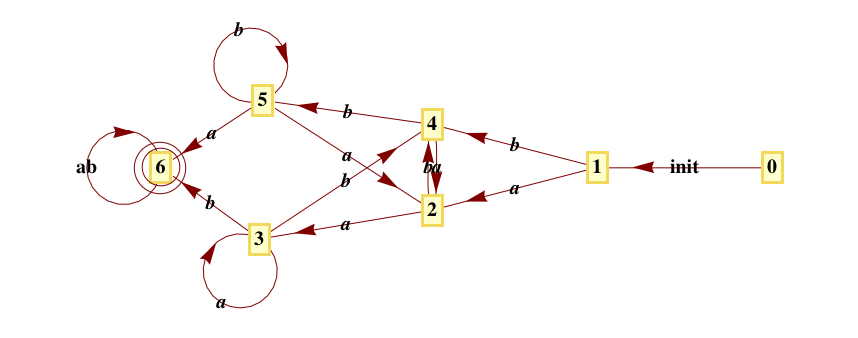
\includegraphics[width=1.0\textwidth]{1-3}
    \caption{All strings over $\{a,b\}$ that contain either $aab$ or $bba$ (or both)}
  \end{figure}

\item
  \begin{fancyquotes}
    (4 points) All strings over $\{a,b\}$ that contain both $aab$ and $bba$
  \end{fancyquotes}
  \begin{figure}[hp]
    \centering
    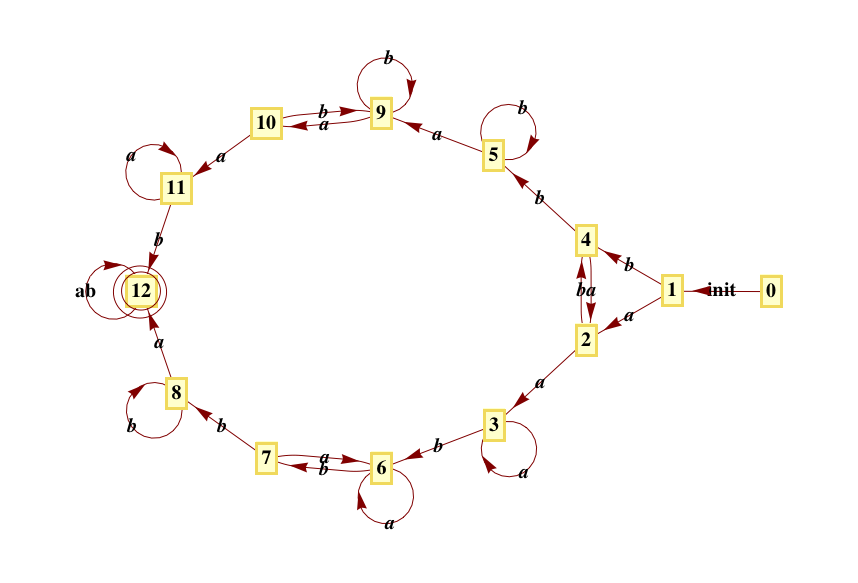
\includegraphics[width=1.0\textwidth]{1-4}
    \caption{All strings over $\{a,b\}$ that contain both $aab$ and $bba$}
  \end{figure}

\item
  \begin{fancyquotes}
    (4 points) All strings over $\{a,b\}$ that contain $aab$ but not $bba$
  \end{fancyquotes}
  \begin{figure}[hp]
    \centering
    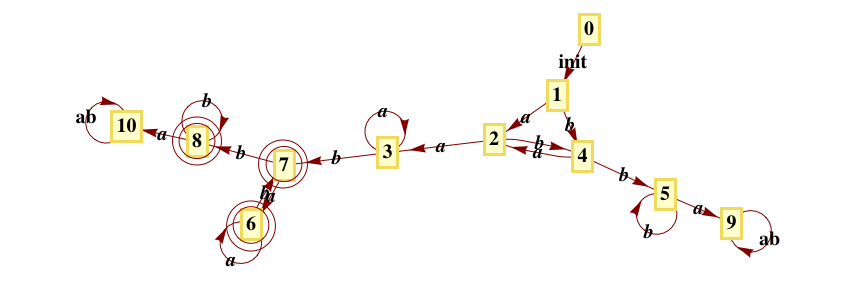
\includegraphics[width=1.0\textwidth]{1-5}
    \caption{All strings over $\{a,b\}$ that contain $aab$ but not $bba$}
  \end{figure}

\end{enumerate}


% -----------------------------------------------------------------------------
% PROBLEM 2
% -----------------------------------------------------------------------------
\section{}

\begin{fancyquotes}
  Give a NFA for each of the following languages:
\end{fancyquotes}

\begin{enumerate}
\item
  \begin{fancyquotes}
    (4 points) $L$ = All strings over $\{a, b, c, d\}$ of length at least 2
    whose second symbol does not appear elsewhere in the string. So
    $bdabc, acbab, bacbd, abcdc \in L$, while $aa, bcabc, abcbc, dd \notin L$
  \end{fancyquotes}
\item
  \begin{fancyquotes}
    (4 points) L = All strings over $\{a, b, c\}$ such that every $a$ is
    followed by either the substring $bcb$ or $ccb$
  \end{fancyquotes}
\end{enumerate}


% -----------------------------------------------------------------------------
% PROBLEM 3
% -----------------------------------------------------------------------------
\section{}

\begin{fancyquotes}
  Give a DFA for the following languages:
\end{fancyquotes}

\begin{enumerate}
\item
  \begin{fancyquotes}
    (4 points) all strings over $\{0\ldots9\}$ that form numbers
    divisible by 7. So, 7, 14, 21, 28, 35, etc are all in the
    language, but 1, 3, 11, 12, 20 are all not in the language. A set
    theory definition (Initial state, final states, transition
    function as a table, etc) is OK, you don't need to draw a
    circle-arrow diagram --- in fact, you probably don't want to draw a
    diagram, it does tend to get a little messy with a larger
    alphabet.
  \end{fancyquotes}

\item
  \begin{fancyquotes}
    (4 points) All strings over $\{a, b, c\}$ that contain an even number
    of a's and an even number of b's and an even number of c's.
  \end{fancyquotes}

\end{enumerate}

\end{document}
